\RCSID $Id: kontsevich.tex,v 1.1 2002/01/10 10:01:51 ri Exp $
%auto-ignore


\chapter{Results of Kontsevich}
\label{cha:kontsevich}

{\Large\itshape Questo capitolo {\`e} ancora \emph{molto} preliminare!}

In the famous paper \cite{witten;intersection-theory}, E.~Witten
related two models of two-dimensional quantum gravity, one based on
matrix integrals and random surfaces, and one which used supersymmetry
to reduce the action integral to a computation of intersection numbers
on the Deligne-Mumford moduli space of stable curves. The partition
function in the first theory was known to obey the KdV differential
equation, so, the belief that both approaches were good models of the
same phenomena led Witten to conjecture that the same equation would
hold also for the partition function in the second theory, namely, for
the generating series of intersection numbers of the moduli space of
curves.

In this form, the conjecture appeared as an infinite hierarchy of
recursion relations among these intersection numbers; Witten himself
proved the first cases using well-known techniques of algebraic
geometry.  Surprisingly, Kontsevich' proof of the full conjecture took
an entirely different route, steering towards Feynman diagrams and a
combinatorial description of the moduli space; what is more, it
provided a model for 2D quantum gravity, which had not been devised
before!  The later paper \cite{witten;kontsevich-model} established
that all three models of 2D quantum gravity are equivalent.

This introductory chapter is an exposition of Kontsevich' Theorem
relating the generating series of intersection numbers on the moduli
space of stable curves with the matrix integral that now bears his
name, as it provides a template for treating intersection theory on
$A_\infty$-classes. I will focus on those techniques that are needed in
the sequel and most suitable to generalization.

This is by no means a complete overview; I refer the interested reader
to the survey papers by Looijenga \cite{looijenga;intersection-theory}
and Dijkgraaf \cite{dijkgraaf;intersection-theory}, which are very
readable yet complete introductions to the results obtained in this
field.


\section{Moduli Spaces of Curves}
\label{sec:moduli-spaces}

Let us recap the main points of the construction of the moduli space
of smooth algebraic curves; the short summary given here tracks
closely the first section of \cite{looijenga;cellular-decomposition},
which has proofs and good references.

Fix integers $g,n\geq0$ such that $2 -2g - n < 0$. Let $S$ be a Riemann
surface of genus $g$ and $P = \{ x_1, \ldots, x_n \}$ a set of $n$ points
in $S$.

Every complex structure  on $S$ determines a conformal structure; let
$\Conf(S)$ be the set of all conformal structures on $S$. 
\begin{definition}\label{dfn:teichmuller}
  The \emph{Teichm{\"u}ller space}
  \begin{equation*}
    \T_{g,n} := \Conf(S) / \Diff^0(S, n)
  \end{equation*}
  is, by definition, the quotient of the set of all conformal metrics on
  $S$ by the set of all diffeomorphisms homotopic to the identity which
  fix the $n$ marked points.
\end{definition}
Every set $P$ of marked points can be carried into another chosen one
$P'$ by a diffeomorphism $\phi \in \Diff^0(S, n)$ --- therefore,
$\Diff^0(S, n)$ depends only on $n$ and not on $P$, cf.
\cite{krushkal;riemann-surfaces}. The Teichm{\"u}ller space $\T_{g,n}$ is
an analytic space and is homeomorphic to a convex domain in $\setC^{3g -
  3 + n}$.

\begin{definition}\label{dfn:mapping-class-group}
  The \emph{mapping class group} $\Gamma_{g,n}$ is defined by:
  \begin{equation*}
    \Gamma_{g,n} := \Diff^+ (S, n) / \Diff^0(S, n).
  \end{equation*}
  It is the set of connected components of the group $\Diff^+(S, n)$ of
  all diffeomorphisms that preserve orientation and fix marked points.
\end{definition}

The topological space $\M_{g,n} := \T_{g,n} / \Gamma_{g,n}$ parameterizes
complex structures on $S$, up to orientation-preserving
diffeomorphisms fixing the $n$ marked points.
\begin{remark}
  One may instead consider equivalence classes of $n$-punctured
  surfaces $S$ (i.e., with $n$ points \emph{removed}) by bianalytic
  mappings. In the event, this moduli space turns out to be the same
  $\M_{g,n}$; this alternate description will occasionally be
  useful.
\end{remark}
\begin{remark}
  Conversely, one may want to keep the complex structure on $S$ fixed,
  while actually moving the points $x_1, \ldots, x_n$; still, this
  \emph{is} a way of varying the complex structure on $(C; x_1, \dots,
  x_n)$. This approach leads to the construction of $\M_{g,n}$
  by equivalence classes of triples $(C, x, f)$ where $C$ is a complex
  curve, $x: \{1, \ldots, n\} \longrightarrow C$ a marking of points,
  and $f: C \to S$ a homeomorphism.
\end{remark}

Since $\T_{g,n}$ is an analytic variety and $\Gamma_{g,n}$ acts
discontinuously with finite stabilizers, $\M_{g,n}$ inherits a
structure of analytic orbifold of complex dimension $3g - 3 + n$.


\subsection{Moduli Space of Stable Curves}
\label{sec:moduli-space-stable}

Deligne and Mumford \cite{deligne-mumford} showed that $\M_{g,n}$ has
a projective compactification $\Mbar_{g,n}$; this space can be
described as the moduli space of stable curves of arithmetic genus
$g$.
\begin{definition}
  A stable complex curve $C$ is a complete connected curve such that:
  \begin{enumerate}
  \item $C$ has only nodal singularities;
  \item the marked points $x_1, \ldots, x_n$ are nonsingular points in
    $C$;
  \item the pair $(C; x_1, \ldots, x_n)$ has a \emph{finite} automorphism
    group.
  \end{enumerate}
\end{definition}
Equivalently, this last condition can be expressed by saying that: 1)
any rational component of the normalized curve $\tilde C$ must contain
at least 3 special points (that is, marked points or singular points);
2) any component of genus $1$ must contain at least 1 special point.
\begin{definition}
  Let $C$ be a stable curve, with $\nu$ irreducible components and
  $\delta$ nodal points. Let $\{C_j\}_{j=1, \dots, \nu}$ be the
  irreducible components of $C$ and $g_{C_j}^{}$ the geometric genus
  of $C_j$.  The arithmetic genus of $C$ is defined by the equation:
  \begin{equation*}
    p_C^{} := \bigl({\textstyle \sum_{j=1}^\nu} g_{C_j}^{} \bigr) + \delta - \nu + 1.
  \end{equation*}
\end{definition}

Informally, stable curves are constructed by attaching smooth curves
``by the nodes'', such that the arithmetic genus be $g$ and the total
number of punctures be $n$.


\section{Witten's conjecture and Kontsevich' theorem}
\label{sec:witten-classes}

\begin{definition}
  The line bundle $\Lb_i \to \Mbar_{g,n}$ is defined by the requirement
  that the fiber over $(C; x_1, \ldots, x_n)$ be the cotangent space
  $T^*_{x_i} C$.
\end{definition}
These $\Lb_i$'s are bundles in a orbifold sense: their first Chern
classes are rational cohomology classes.
\begin{definition}
  The Witten's classes are the rational cohomology classes $\psi_i :=
  c_1({\Lb}_i)$.
\end{definition}

For non-negative integers $\nu_1, \ldots, \nu_n$, define
\begin{equation}
  \label{eq:intersection-index}
  \langle \tau_{\nu_1} \cdots \tau_{\nu_n} \rangle_{g,n} := \int_{\Mbar_{g,n}} \psi_1^{\nu_1} \cdots \psi_n^{\nu_n}.
\end{equation}
The integral on right-hand side can be nonzero only if $v_1 + \cdots + \nu_n = 3g
- 3 + n$; notice that $g$ is uniquely determined, given $n$ and
$\nu_1$, \ldots, $\nu_n$. Therefore, we drop the subscript $g,n$ in
the equation above, since no confusion can occur. Mumford
\cite{mumford;enumerative-geometry} remarked that, by a theorem of
Arakelov,
\begin{equation}
  \label{eq:positive-intersection}
  \langle\tau_{\nu_1} \cdots \tau_{\nu_n}\rangle \geq 0.
\end{equation}

\begin{definition}\label{dfn:F-and-Z}
  The ``free energy'' is the following formal series in an infinite
  number of indeterminates:
  \begin{equation}\label{eq:F-dfn}
    F(t_0, t_1, \ldots) := \sum_{g, n, \nu_1, \ldots, \nu_n} \langle
    \tau_{\nu_1} \cdots \tau_{\nu_n} \rangle t_{\nu_1} \cdots t_{\nu_n}.
  \end{equation}
  
  The ``partition function'' is the formal series 
  \begin{equation}\label{eq:Z-dfn}
    Z(t_*) := \exp F(t_*).
  \end{equation}
\end{definition}

The permutation group $\Perm{n}$ acts trivially on
$\Htop(\Mbar_{g,n})$, so we can introduce the abridged notation:
\begin{equation}
  \label{eq:intersection-index-cpt}
  \langle\tau_0^{d_0} \tau_1^{d_1} \cdots \tau_k^{d_k} \rangle := \langle \underbrace{\tau_0 \cdots
    \tau_0}_{\text{$d_0$ times}} \cdots \underbrace{\tau_k \cdots
    \tau_k}_{\text{$d_k$ times}} \rangle.
\end{equation}
With this proviso, we may rewrite:
\begin{equation}\label{eq:F-dfn-cpt}
  F(t_*) = \sum_{g, d_1, \ldots, d_k} \langle \tau_0^{d_0} \cdots \tau_k^{d_k} \rangle \frac
  {t_0^{d_0} \cdots t_k^{d_k}} {d_0! \cdots d_k!} =: \sum_{g, d_*} \langle \tau_*^{d_*}
  \rangle t_*^{d_*}/d_*!,
\end{equation}
a formula that will occasionally come handy.

Witten \cite{witten;intersection-theory} conjectured that $Z$ satisfies
a certain hierarchy of differential equations (the KdV hierarchy).
Kontsevich \cite{kontsevich;intersection-theory;1992} expressed $Z$ as
an asymptotic expansion of a certain matrix integral; this is enough
to prove Witten's conjecture
(\cite{kontsevich;intersection-theory;1992},
\cite{witten;kontsevich-model}). Let us state this assertion
precisely.

Let $\Hn := \Hermitian[N]$ be the space of all $N \times N$ Hermitian
matrices; let $\Lambda \in \Hn$ be a positive definite diagonal
Hermitian matrix, that is,
\begin{equation*}
  \Lambda = \text{diag}( \Lambda_1, \ldots, \Lambda_N ),
\end{equation*}
for real numbers $\Lambda_i > 0$. The \emph{Miwa coordinates} are the
functions defined by:
\begin{equation*}
  t_i (\Lambda) := -(2i-1)!! \tr \Lambda^{-2i-1}.
\end{equation*}
For any given $N$, coordinates $t_1$, \ldots, $t_N$ are independent on
$\Hermitian[N]/U(N)$. Now, $\Hn$ is a finite-dimensional real vector
space, therefore, there is a naturally defined translation-invariant
measure $\ud X$. Let $\ud\mu_\Lambda(X)$ be the Gaussian measure associated
to $\exp ( -1/2 \tr \Lambda X^2)$, that is,
\begin{equation*}
  \ud \mu_\Lambda(X) := \frac{1}{C} \cdot \exp ( -1/2 \tr \Lambda X^2)
  \ud X, \qquad C := \int_\Hn  \exp ( -1/2 \tr \Lambda X^2) \ud X.
\end{equation*}

\begin{definition}\FIXME{Togliere?}
  A formal series $\sum a_j t^j$ is an asymptotic expansion of a real
  function of a real variable $f(t)$ 
  at a point $t_0$ iff
  \begin{equation*}
    \lim_{t \to t_0} t^{-(k+1)} \bigl( f(t) - {\textstyle\sum_0^k a_j t^j}
    \bigr) = a_{k+1}.
  \end{equation*}
\end{definition}
If an asymptotic expansion exists, it is unique. The definition
generalizes easily to functions of many variables; however, the
asymptotic expansion of a function depends on its domain, that is, $f$
and its restriction to a smaller domain may not have the same
asymptotic expansion at one point $t_0$.
\begin{theorem}[Kontsevich]
  \label{thm:kontsevich}
  The formal series $Z(t_0(\Lambda), t_1(\Lambda), \ldots)$ is an asymptotic
  expansion of
  \begin{equation*}
    \label{eq:K}
    \int_{\Hermitian[N]} \exp(\I/6 \tr X^3) \ud\mu_\Lambda(X),
  \end{equation*}
  when $\Lambda^{-1} \to 0$ and $N \gg 0$.
\end{theorem}
Therefore, one can compute $F(t_0(\Lambda), t_1(\Lambda), \ldots)$ through 
\begin{equation*}
  F(t_0(\Lambda), t_1(\Lambda), \ldots) \asymp \log     \int_\Hn \exp({\I}/{6} \tr X^3) \ud\mu_\Lambda(X).
\end{equation*}
The intersection numbers of $\Mbar_{g,n}$ can be computed by choosing
$N > 3g - 3 + n$; in the limit $N \to \infty$ we retrieve information on
all moduli spaces. 

%%Kontsevich' proof is a ingenious mix of two main ingredients:
%%\begin{enumerate}
%%\item a triangulation of $\M_{g,n}$, whose cells are labeled by ribbon
%%  graphs;
%%\item the expansion of the integral \ref{eq:K} in Feynman graphs.
%%\end{enumerate}
%%So, these are the topics we are going to discuss next.


\section{A combinatorial model of $\M_{g,n}$}
\label{sec:mgn-comb}

\FIXME{Questa sezione sta meglio in una appendice? Meglio tagliarla
  drasticamente?}
String field theory attempts to explain properties of the fundamental
particles by treating them like ``small'' closed strings. When
point-like particles move in space-time, they draw trajectories; when
strings move, they draw ``tubes''; when tubes join, they form a
punctured surface. This simple idea is the link between string theory
and the moduli space of curves. 

Let $S$ be an $n$-punctured Riemann surface (i.e., a Riemann surface
with $n$ points removed); $S$ retracts onto a graph. This graph is not
uniquely determined.
\begin{figure}[bt]
  %% Figura sphere3.fig
  \centering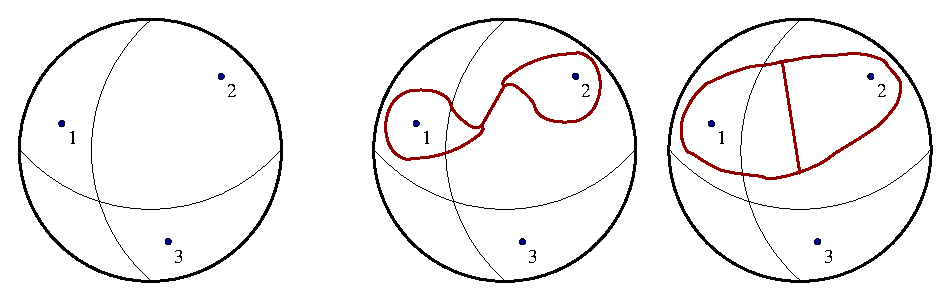
\includegraphics[width=\textwidth]{sfera3}
  \caption{A thrice punctured sphere and two inequivalent
    deformation retracts.} 
  \label{fig:sphere-retracts}
\end{figure}
We look forward to refining this correspondence: let us introduce more
structure on the graph.
\begin{definition}
  \label{dfn:metric-ribbon-graphs}
  A metric ribbon graph is the data of a type (0,0) ribbon graph (see
  \csref{dfn:ribbon-graphs}) equipped with a real positive number
  $\ell_\alpha$ for each edge $\alpha$.
\end{definition}

One can use the cyclic order to ``fatten'' edges of a graph $\Gamma$ into
thin ribbons\footnote{Hence the names ``ribbon graph'' and
  ``fatgraph''.}  (see \csref{fig:fattening-edges}), so to obtain a
compact oriented Riemann surface with boundary $\tilde S(\Gamma)$.
Viceversa, any graph $\Gamma$, embedded in a oriented Riemann surface,
inherits a cyclic order from the orientation.
\begin{figure}[htbp]
  \begin{equation*}
    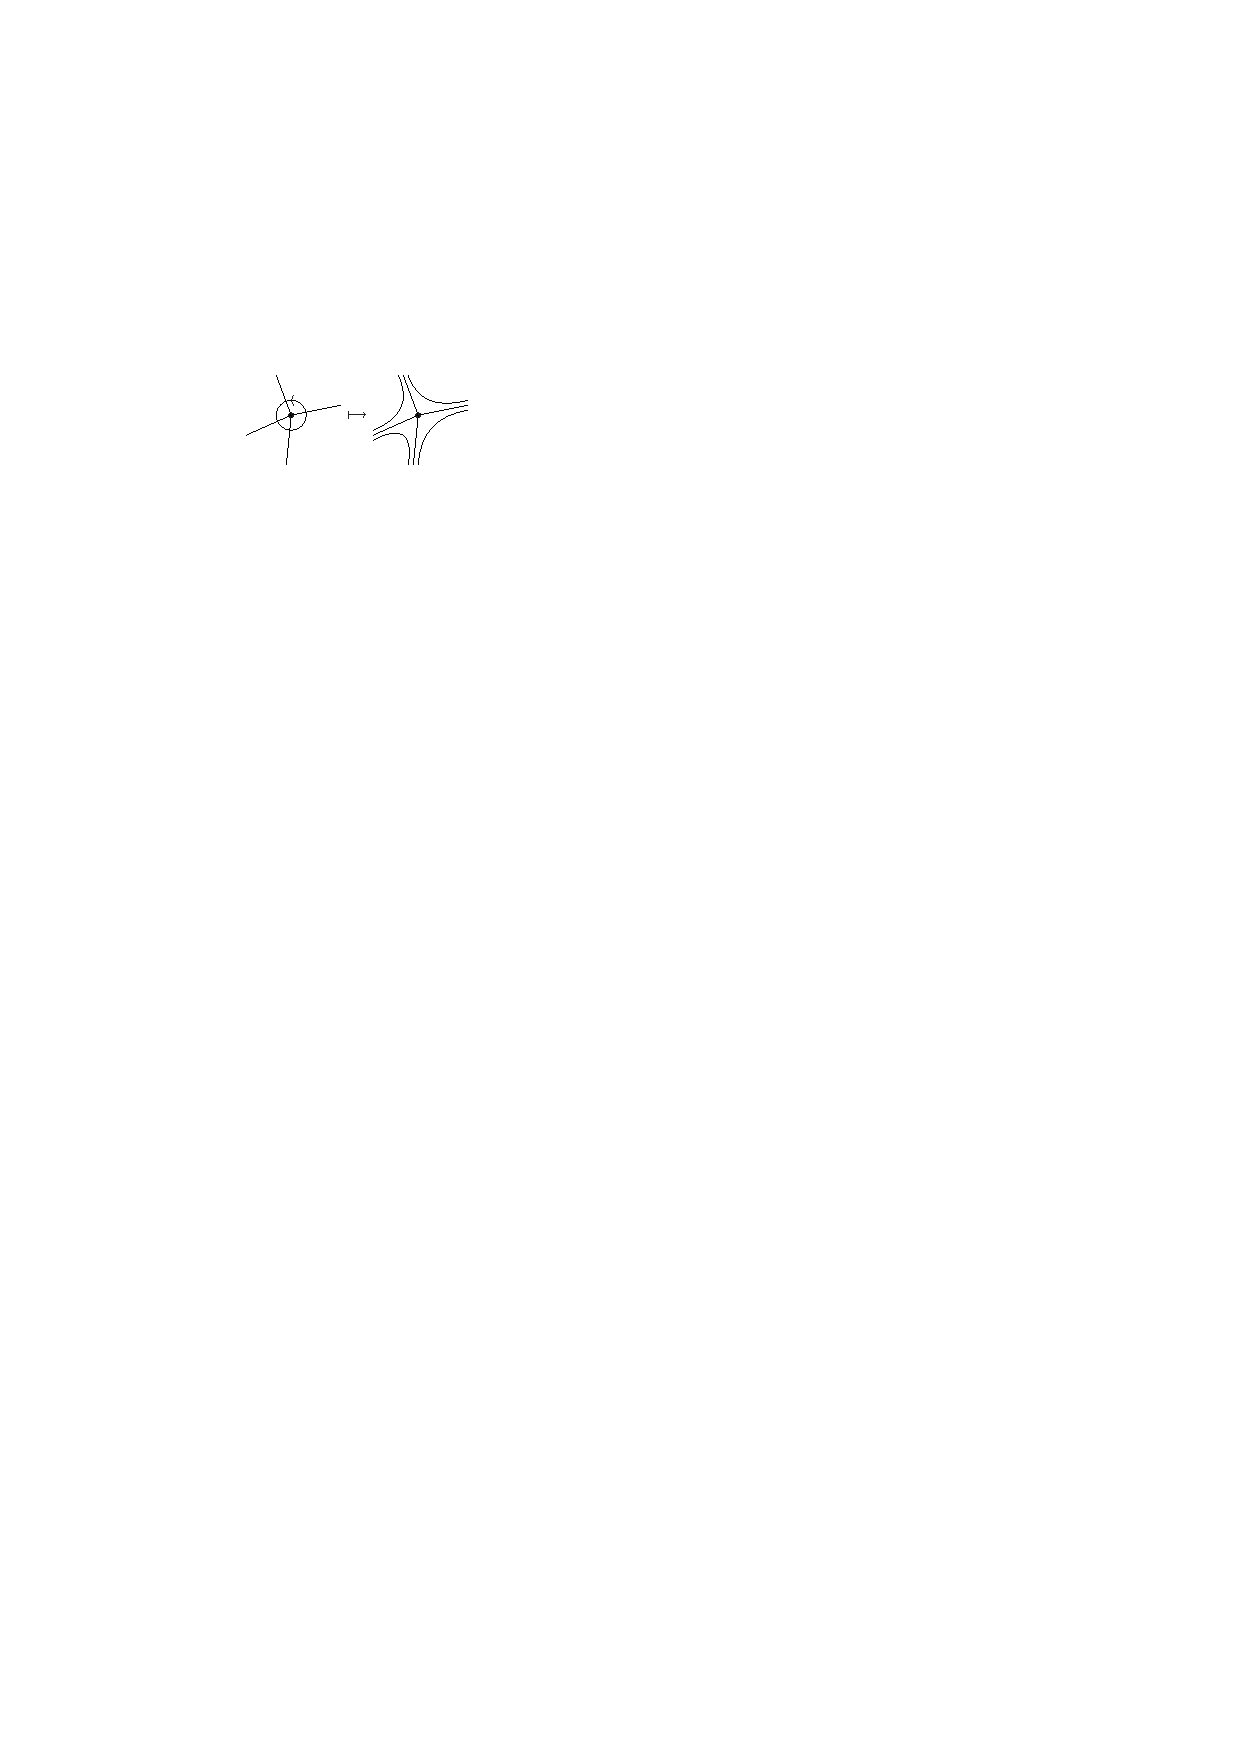
\includegraphics{fatten}
  \end{equation*}
  \caption{Fattening edges at a vertex with cyclic order.}
  \label{fig:fattening-edges} 
\end{figure} 
Now glue punctured disks alongside the boundary of $\tilde S(\Gamma)$ to
get a punctured Riemann surface $S(\Gamma)$. Obviously,
\begin{equation*}
  \chi(\Gamma) = \chi(S(\Gamma)) = 2 - 2g - n,
\end{equation*}
so we can define, for a ribbon graph $\Gamma$, the \emph{genus} $g$ and the
\emph{puncture number} $n$, as given by the above relation.

Notice that this fattening procedure actually selects some homological
$1$-cycles in $\Gamma$, those corresponding to the boundary components of
$\tilde S(\Gamma)$. By abuse of language, we shall call these $1$-cycles
``boundary components'' or ``holes'', for short.

Denote $\Vertices{\Gamma}$, $\Edges{\Gamma}$ and $\Holes{\Gamma}$ the
sets of vertices, edges and holes of a graph $\Gamma$. It will be
convenient to identify a hole $\beta$ with the set of edges it is made
of, and a vertex $\gamma$ with the set of edges incident to it.


\subsection{A complex structure on $S(\Gamma)$}
\label{sec:atlas}
Let us give the topological Riemann surface $S(\Gamma)$ a complex
structure, by means of a triangulation and an analytic atlas.

In the course of the construction of $S(\Gamma)$, two punctured disk
have been glued on the sides of an edge $\alpha \in \Edges{\Gamma}$: call
them $\alpha^+$ and $\alpha^-$. Let $T_\alpha^+$ and $T_\alpha^-$ be the triangles
delimited by $\alpha$ and the radii joining endpoints of $\alpha$ with the
puncture of $\alpha^\pm$. The collection $\{T_\alpha^\pm : \alpha \in \Edges{\Gamma}\}$
is a triangulation of $S(\Gamma)$.

Define an atlas of $S(\Gamma)$:
\begin{itemize}
\item for any edge $\alpha$, put $V_\alpha := (T_\alpha^+ \cup T_\alpha^-)^\circ$;
\item for any hole $\beta$, put $V_\beta := \bigl( \bigcup_{\alpha} T_\alpha \bigr)^\circ$
  for all $\alpha$ bounding $\beta$;
\item for any vertex $\gamma$, put $V_\gamma := \bigl( \bigcup_\alpha T_a^\pm \bigr)^\circ$
  for all $\alpha$ incident to $\gamma$.
\end{itemize}
\begin{figure}[btp]
    %% Figura atlas.fig
  \centering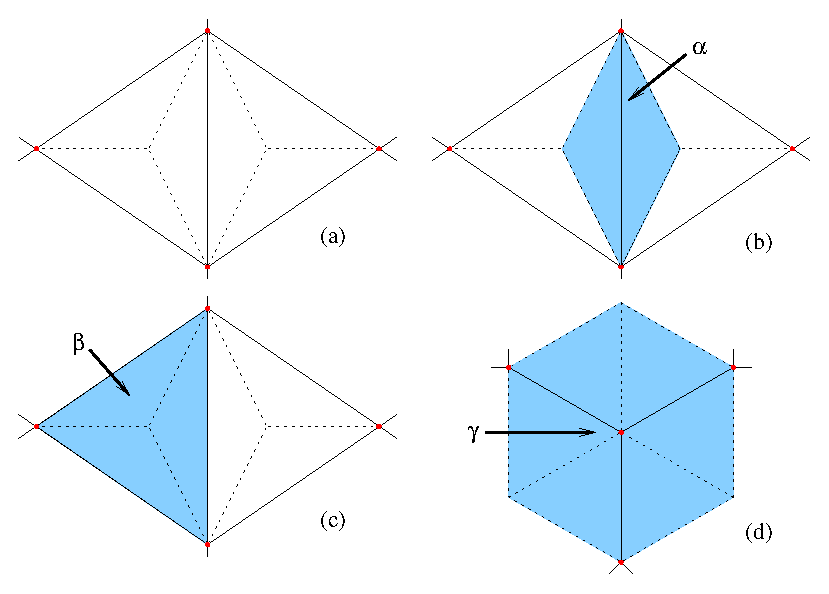
\includegraphics[width=\textwidth]{atlas}
  \caption{The open sets building an atlas of $S(\Gamma)$: (a) the
    triangulation built from a graph $\Gamma$; (b) the neighborhood
    $V_\alpha$ of an edge $\alpha$; (c) the neighborhood $V_\beta$ of a hole
    $\beta$; (d) the neighborhood $V_\gamma$ of a vertex $\gamma$.}
  \label{fig:atlas}
\end{figure}

Define charts on the open sets $V$ (see Figure~\ref{fig:charts}):
\begin{itemize}
\item for any edge $\alpha$, pick a homeomorphism $f_\alpha: V_\alpha \to \{ z \in \setC
  : 0 < \Re z < \ell_\alpha \}$;
\item for any hole $\beta$, bounded by edges $\alpha_1$, $\alpha_2$ and $\alpha_3$,
  pick a homeomorphism $f_\beta: V_\beta \to \{ \abs{z} < \rho \}$, where $\rho =
  (\ell_{\alpha_1} + \ell_{\alpha_2} + \ell_{\alpha_3}) / 2\pi$.
\item for any vertex $\gamma$, pick a homeomorphism $f_\gamma: V_\gamma \to \setC$.
\end{itemize}
\begin{figure}[htbp]
    %% Figura charts.fig
  \centering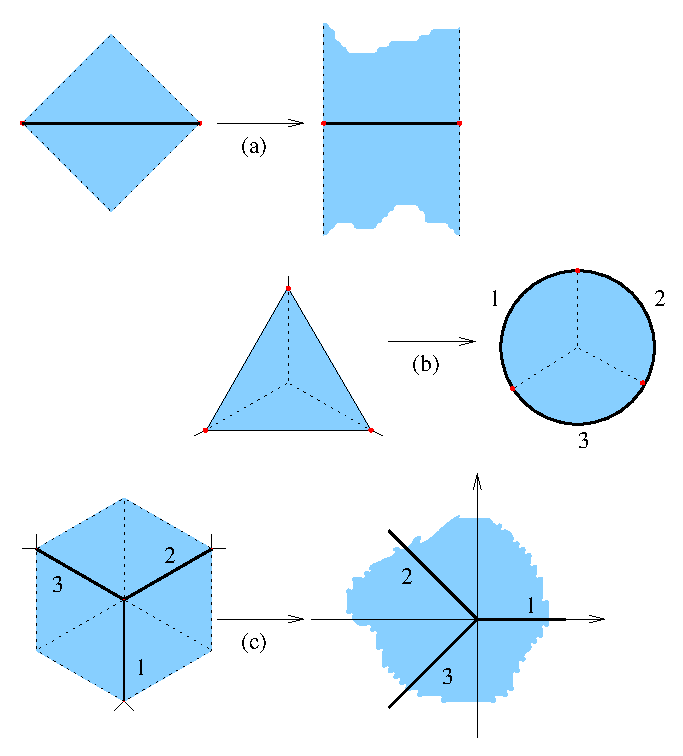
\includegraphics{charts}
  \caption{Local charts on the atlas: (a) any open set $V_\alpha$
    maps to a strip in the complex plane; (b) any open set $V_\beta$
    maps to a disk; (c) any open set $V_\gamma$ maps to the complex
    plane itself.}
  \label{fig:charts}
\end{figure}
These choices are subject to the condition that transition functions
satisfy the following:
\begin{itemize}
\item if $\alpha$ is an edge bounding the hole $\beta$, then $f_\beta \circ
  f_\alpha^{-1} = \exp (2\pi\I z / p_\beta)$ with $p_\beta := \sum_{\alpha \in \beta} \ell_\alpha$
  (\emph{perimeter} of the hole $\beta$);
\item if $\alpha$ is incident to a vertex $\gamma$, then $f_\gamma \circ f_\alpha^{-1} =
  c \cdot z^{2/(m+2)}$, up to a complex constant of modulus $1$, where
  $m$ is the valence of the vertex $\gamma$.
\end{itemize}

In the end, we have come upon a complex analytic structure on
$S(\Gamma)$, which depends on the perimeters $p_1, \ldots, p_n$ of holes $\beta_1,
\ldots, \beta_n$. By varying these (real positive) parameters, one can vary
the complex structure on $S(\Gamma)$; this will allow for an alternative
construction of the moduli space $\M_{g,n}$.


\subsection{The Strebel construction}
\label{sec:strebel}
A theorem proved by K. Strebel in the 1960's provides an inverse
route to the construction of smooth complex curves from ribbon
graphs. 

\begin{definition}
  A quadratic differential $q$ on a Riemann surface $S$ is a
  (meromorphic) section of $(T^*)\tp2$.
\end{definition}
The set of vectors in $T_zS$ on which $q$ takes real non-negative
values form a real line in $T_zS$: therefore, they make up a foliation
on $S$. The non compact leaves together with zeroes of $q$ form the
``critical locus'' of $q$.

Every quadratic differential $q$ induces a metric (away from the
critical locus) by $ds^2 = \abs{q(z)} \cdot \abs{\ud z}$.

\begin{theorem}[Strebel, {\cite[Theorem 23.2 and
    23.5]{strebel;quadratic-differentials;1983}}] For all complex
  analytic curve $S$, with $n$ marked points $x_1, \ldots, x_n$, and any
  assignment of real positive numbers $p_1, \ldots, p_n$, there exists one
  and only one meromorphic quadratic differential $q$ such that:
  \begin{enumerate}
  \item the critical locus of $q$ is a graph $\Gamma$ embedded in $S$;
  \item the poles of $q$ reside in the marked points $x_1, \ldots, x_n$
    with second residue $p_1, ..., p_n$;
  \item every compact leaf rounding $x_i$ has length $p_i$ in the flat
    metric induced by $q$.
  \end{enumerate}
\end{theorem}
The critical graph $\Gamma$ inherits a structure of ribbon graph with
metric from the ambient surface $S$; the length of an edge $\alpha$ is the
one measured in the metric induced by the quadratic
differential. Furthermore, Strebel's theory states that $\Gamma$ has a
vertex of valence $k+2$ where $q$ has a zero of order $k$, therefore,
vertices of $\Gamma$ have valence $\geq3$.

Since the markings $x_1, \ldots, x_n$ are \emph{ordered}, $\Gamma$ has an
additional structure of \emph{numbered} graph, that is, it is endowed
with a bijection $h: \Holes{\Gamma} \to \{1, \ldots, n\}$. 
\begin{definition}
  \label{dfn:strebel-graphs}
  Define a category $\Strebel[g,n]$, whose objects are metric numbered
  ribbon graphs with genus $g$ and $n$ holes, all whose vertices have
  valence $\geq3$ (call them ``Strebel graphs'', for short) .  Morphisms
  $\Gamma \to \Gamma'$ are compositions of graph isomorphisms and contractions of
  an edge $\alpha \in \Edges{\Gamma}$.
\end{definition}

Let $\Gamma$ be a Strebel graph of genus $g$ with $n$ holes.  A topological
cell $\Delta_\Gamma \subseteq \M_{g,n}$ is spanned when varying the metric data
$(\ell_\alpha)_{\alpha \in \Edges{\Gamma}}$; gluing these cells one recovers the
whole $\M_{g,n}$. We present here a quick construction, apparently due
to Kontsevich \cite{kontsevich;intersection-theory;1992}.

Call a set $X \subseteq \Edges{\Gamma}$ negligible whenever it is \emph{not} the
support of any non-trivial homological cycle.  Define
\begin{equation*}
  \label{eq:kontsevich-3}
  M(\Gamma) := \{ \ell: \Edges{\Gamma} \to \setR_{>0} | \text{the zero set of $\ell$ is negligible}\}.
\end{equation*}
It is a contravariant functor from the category of Strebel graphs to
the category of topological spaces: if $\Gamma'$ is obtained from $\Gamma$ by
contracting the edge $\alpha_0$, then
\begin{equation*}
  M(\Gamma') = \{ \ell \in M(\Gamma) | \ell_\alpha = 0 \}.
\end{equation*}
\begin{definition}
  The combinatorial moduli space of smooth algebraic curves is the
  direct limit of the functor $M$:
  \begin{equation*}
    \Mcomb_{g,n} := \varinjlim M(\Gamma),
  \end{equation*}
  with $\Gamma$ in the category $\Strebel[g,n]$ of Strebel graphs.
\end{definition}
\begin{remark}
  $\Mcomb_{g,n}$ is obtained by gluing orbicells $M(\Gamma)$ (quotient of
  a topological cell by $\Aut \Gamma$) alongside the boundary (if $\Gamma'$ is a
  contraction of $\Gamma$, then $M(\Gamma')$ is a face of $M(\Gamma)$). Therefore,
  $\Mcomb_{g,n}$ is a orbifold.
\end{remark}

It is easy to check that any $[\Gamma, \ell] \in \Mcomb_{g,n}$ has a unique
representative such that $\ell_\alpha > 0$ for all $\alpha \in \Edges{\Gamma}$.
The perimeter maps $p_\beta: \Mcomb_{g,n} \to \setR_{>0}$ are well-defined;
write $p_j$ for the perimeter of the $j$-th hole.

The construction of $\Mcomb_{g,n}$ can be done with slightly changed
rules: if we define a set $X \subseteq \Edges{\Gamma}$ to be negligible iff it
does not contain all edges bounding a hole, then we can define a
contrafunctor $\overline{M}(\Gamma)$ and a topological space:
\begin{equation*}
  \label{eq:kontsevich-4}
  \Mbarcomb_{g,n} := \varinjlim \overline{M}(\Gamma).
\end{equation*}
$\Mbarcomb_{g,n}$ turns out to be a compactification of the orbifold
$\Mcomb_{g,n}$. 

\begin{theorem}[Mumford, Harer, Penner, Thurston;
  \cite{looijenga;cellular-decomposition}] 
  The Strebel construction defines morphisms
  \begin{equation*}
    \M_{g,n} \times \setR_{>0}^n \to \Mcomb_{g,n}, \qquad \Mbar_{g,n} \times
    \setR_{>0}^n \to \Mbarcomb_{g,n}.
  \end{equation*}
  The first of these is a homeomorphism and, more, an orbifold
  equivalence. The inverse map
  \begin{equation*}
    \Mcomb_{g,n} \to \M_{g,n} \times \setR_{>0}^n \to \setR_{>0}^n
  \end{equation*}
  is the perimeter map $\pi := (p_1, \ldots, p_n)$.  
\end{theorem}

For any given $p^\circ = (p_1^\circ, \ldots, p_n^\circ) \in \setR_{>0}^n$, the fiber
$\pi^{-1}(p^\circ)$ is isomorphic to $\M_{g,n}$, thus, $\pi$ induces a
triangulation of $\M_{g,n}$.

The cell $M(\Gamma)$ has real dimension $\card{\Edges{\Gamma}}$; therefore,
cells of maximal dimension are given by graphs with all vertices of
valence $3$. The union of these cells is a dense subset of
$\Mcomb_{g,n}$ with non-void interior.


\section{Kontsevich' calculations}
\label{sec:calculation}

Kontsevich' praised calculation provides the bridge between the
combinatorial approach to the geometry of moduli spaces and the
Feynman diagrams theory of matrix integrals. In view of later
applications \cite{witten;kontsevich-model}, this should be
regarded as the very important result in Kontsevich' proof of Witten's
conjecture.


\subsection{Combinatorial expression of Witten's classes}
\label{sec:wittens-classes-comb}
\FIXME{Tutta questa sezione pu{\`o} ridursi al solo \csref{thm:comb-bundle}?}
Let $C_N$ be the cyclic group of order $N$. Define $B_N := \setR^N / C_N$
to be the orbicell of sequences $[l_1, \ldots, l_N]$ of non-negative real
numbers modulo cyclic permutations, endowed with the quotient
topology. There exist $N+1$ natural inclusion maps $\iota_j: B_N \ni [l_1,
\ldots, l_N] \mapsto [l_1, \ldots, l_{j-1}, 0, l_j, \ldots, l_N] \in B_{N+1}$; these
make $\{B_N, \iota\}$ into an inductive family of topological spaces.
Finally, define
\begin{equation*}
  B := \varinjlim B_N.
\end{equation*}
Every point of $B$ has a unique representative $[l_1, \ldots, l_N]$
enjoying $l_j > 0$ for all $j$. It is convenient to introduce
``barycentric'' coordinates $[p; s_1, \ldots, s_N]$ given by $p := \sum l_j$
and $s_j := l_j/p$.

Define $U_N := \{ (p; \Theta) | p>0, \ \Theta\subseteq S^1, \card{\Theta} = N\}$; give it
the subspace topology of $(S^1)^N$. The group $S^1$ acts on every
$U_N$, and there are surjections $f_\sigma$, for $\sigma \in C_N$:
\begin{multline*}
  E_N := \{ (p; \theta_1, \ldots, \theta_N) | 0\leq \theta_1 < \ldots < \theta_N < 1\} \ni (p;
  \theta_1, \ldots, \theta_N) 
  \\
  \stackrel{f_\sigma}{\longmapsto} [p; \E^{\I\theta_1}, \ldots,
  \E^{\I\theta_N}] \in U_N.
\end{multline*}
Put $U_{\leq N} := \bigcup_{j \leq N} U_j$; the inclusions $U_{\leq N} \hookrightarrow U_{\leq
  N+1}$ define an inductive family. Finally, define:
\begin{equation*}
  E := \varinjlim U_{\leq N}.
\end{equation*}
The coordinate patch $E^\sigma_N := (E_N, f_\sigma)$ covers the stratum $U_N
\subseteq E$.

Define projection maps $E^\sigma_N \to B_N$ by 
\begin{equation*}
  E_N^\sigma \ni (p; \theta_1, \ldots, \theta_N) \mapsto [p; \theta_2 - \theta_1, \theta_3 - \theta_2, \ldots, 1
  + \theta_1 - \theta_N] \in B_N;
\end{equation*}
they can be glued into a continuous surjection $\ell: E \to B$, whose
fibers are the orbits of the action of $S^1$ on $E$. It is easy to
check that the spaces $B$ and $E$ are contractible and that $E$ is an
$S^1$-bundle on $B$.
\begin{lemma}
  \label{thm:comb-bundle}
  There exists a differential $1$-form $\alpha$ on $E$ such that:
  \begin{enumerate}
  \item on any patch $E^\sigma_N$, $\alpha$ is given by
    \begin{equation*}
      \alpha := \sum_{j=1}^N s_j \ud\theta_j, \qquad s_j= \theta_{j+1} - \theta_j, \ s_N = 1 +
      \theta_1 - \theta_N;
    \end{equation*}
  \item $\alpha$  restricts to the angle form on the fibers of $\ell$.
  \item   the differential $\ud\alpha$ relates to the first Chern class of $E$
    according to $\ud\alpha = -s^*c_1(E)$;
  \item the differential $\ud\alpha$ is the pull-back on $E$ of a $1$-form $\omega$
    on $B$, defined by:
    \begin{equation*}
      \omega = \sum_{1\leq j\leq k\leq N-1} \ud s_j \land \ud s_k.
    \end{equation*}
  \end{enumerate}
\end{lemma}
\begin{proof}
  Items 1)--2) may be proved by direct calculation; 3) is a standard
  result: consult, for instance, \cite{bott-tu}; finally 4) can be
  seen by induction on $N$.
\end{proof}

Now, the turnkey observation is that points in $B$ may be regarded as
circles with $N$ points marked, that is, ribbon graphs with only
2-valent vertices; so, we can define maps $b_j: \Mcomb_{g,n} \to B$ which
send the $j$-th hole $\beta$ (made of edges $\alpha_1$, \ldots, $\alpha_N$) to the
point $[\ell_{\alpha_1}, \ldots, \ell_{\alpha_N}] \in B_N \subseteq B$. 
\begin{theorem}[Kontsevich, {\cite[Theorem
    2.3]{kontsevich;intersection-theory;1992}}]
  The map $\M_{g,n} \times \setR^n \to B$, which is the composition of the
  maps $b_j$ with the isomorphism $\M_{g,n} \times \setR^n \simeq
  \Mcomb_{g,n}$, extends continuously to $\Mbar_{g,n} \times \setR^n$. The
  inverse image of the bundle $E \to B$ under $b_j$ is naturally
  isomorphic to the $S^1$-bundle associated with the complex line
  bundle ${\Lb}_j$. The pull-back $\omega_j$ of the form $\omega$ (defined in
  \csref{thm:comb-bundle}) under $b_j$ represents the class
  $c_1({\Lb}_j)$. 
\end{theorem}


\subsection{Kontsevich' Main Identity}
\label{sec:KMI}

Results from the previous section allow us to write
\begin{equation}
  \label{eq:kontsevich-6}
  \langle \tau_{\nu_1} \cdots \tau_{\nu_n} \rangle = \int_{\pi^{-1}(p^\circ_*)} \omega^{\nu_1} \land \cdots
  \land \omega^{\nu_n},
\end{equation}
but actually, as Kontsevich proved, one can draw a much stronger
conclusion. 

\begin{theorem}[Kontsevich' Main Identity]
  Let $\RG[g,n]$ be the set of isomorphism classes of numbered
  ribbon graphs with genus $g$ and $n$ boundary components. If
  $\alpha$ is an edge of a graph $\Gamma \in \RG[g,n]$, let $\alpha^+$
  and $\alpha^-$ be the \emph{numbers} assigned to the two holes on
  the sides of $\alpha$. For complex indeterminates $\lambda_1$,
  \ldots, $\lambda_N$, the following relation holds:
  \begin{multline*}
    \sum_\nu \langle \tau_{\nu_1} \cdots \tau_{\nu_n} \rangle \prod_{j=1}^n \frac {(2\nu_j - 1)!!}
    {\lambda_j^{2\nu_j + 1}} = \sum_{\Gamma \in \RG[g,n]} \frac
    {2^{-\card{\Vertices{\Gamma}}}} {\card{\Aut \Gamma}} \prod_{\alpha \in \Edges{\Gamma}}
    \frac {2} {\lambda_{\alpha^+} + \lambda_{\alpha^-}}, 
    \\ \sum \nu = 3g - 3 + n.
  \end{multline*}
\end{theorem}
\begin{proof}
  Define a differential $2$-form on $\Mbarcomb_{g,n}$ by $\Omega := \sum
  p_j^2 \omega_j$. Recall that the metric data $(\ell_\alpha)_{\alpha \in \Edges{\Gamma}}$
  define local coordinates on the orbicell $M(\Gamma)$; it is easy to check
  that the restriction of $\Omega$ to the fibers of $\pi$ is non-degenerate
  and has constant coefficients in the coordinates $\ell_\alpha$. 
  
  Therefore, $\Omega^q$, with $q := 3g -3 + n = \dim \M_{g,n}$, is a
  volume form on the fibers of $\pi$.  The product $\Omega^q/q! \times
  dp_*$ is a volume form on the whole $\Mcomb_{g,n}$ and one can check
  that the ratio of measures
  \begin{equation*}
    \rho := (\Omega^q/q! \times {dp_1 \land \cdots \land dp_n}) / (d\ell_1 \land \cdots \land d\ell_N) 
  \end{equation*}
  is a \emph{constant}, independent of $\Gamma$ (that is, local expression
  in a cell $M(\Gamma)$), and depending only on $g$ and $n$; more precisely,
  \begin{equation*}
    \rho = 2^{2n + 5g - 5} = 2^{q - \card{\Vertices{\Gamma}} + \card{\Edges{\Gamma}}}.
  \end{equation*}
  The proof of this last fact is quite technical and intricate: see
  \cite[Appendix C]{kontsevich;intersection-theory;1992}.

  Consider the integral
  \begin{equation*}
    I := \int_{\Mbarcomb_{g,n}} \Omega^q/q! \cdot \exp(-\sum \lambda_j p_j) dp_*.
  \end{equation*}
  On the one hand, from formula
  \begin{equation*}
    \int_{\pi^{-1}(p^\circ_*)} \Omega^q/q! = (1/q!) \cdot \int_{\pi^{-1}(p^\circ_*)} \bigl( p_1^2
    c_1({\Lb}_1) + \cdots + p_n^2 c_1({\Lb}_n) \bigr)^q,
  \end{equation*}
  and \eqref{eq:kontsevich-6}, one can compute:
  \begin{equation}
    \label{eq:8}
    I = \sum_\nu \langle \tau_{\nu_1} \cdots \tau_{\nu_n} \rangle \prod_{j=1}^n (2\nu_j)!!
    \lambda_j^{-2\nu_j -1}, \qquad \sum \nu_j = q.
  \end{equation}

  On the other hand, since the ratio $\rho$ is constant on all of
  $\Mcomb_{g,n}$, then 
  \begin{equation*}
    I = \rho \cdot \int_{\Mcomb_{g,n}} \exp(-\sum \lambda_j p_j) \abs{d\ell_1 \land \cdots \land d\ell_N}.
  \end{equation*}
  Since the Strebel triangulation of $\Mcomb_{g,n}$ is indexed by
  ribbon graphs, we can immediately say that the above integral is a
  sum of terms corresponding to ribbon graphs; what is more, since the
  integral can be computed by restricting to an open stratum, we may
  limit the sum to trivalent ribbon graphs only. A little
  combinatorics shows that, for a fixed trivalent ribbon graph
  $\Gamma$,
  \begin{equation*}
    \exp( -{\textstyle \sum} \lambda_j p_j) = \prod_{\alpha \in \Edges{\Gamma}} \exp -\ell_\alpha(\lambda_{\alpha^+} +
    \lambda_{\alpha^-}),
  \end{equation*}
  so that we can finally compute:
  \begin{equation}
    \label{eq:7}
    I = \sum_{\Gamma \in \RG[g,n]} \frac {1} {\card{\Aut \Gamma}} \prod_{\alpha \in
      \Edges{\Gamma}} \frac{1} {\lambda_{\alpha^+} +
      \lambda_{\alpha^-}}.
  \end{equation}

  Multiply by $2^{-q}$ and equate \eqref{eq:7} and \eqref{eq:8} to get
  the thesis.
\end{proof}

Take a formal sum, over all $g,n$, of the LHS of the Main
Identity, and substitute $\Lambda_{j_k}$ for $\lambda_k$: 
\begin{multline}
  \label{eq:KMI-F}
  F(t_0(\Lambda), t_1(\Lambda), \ldots) = \sum_{n, \nu_1, \ldots, \nu_n} 1/n! \langle \tau_{\nu_1}
  \cdots \tau_{\nu_n} \rangle t_{\nu_1}(\Lambda) \cdots t_{\nu_n}(\Lambda)
  \\
  = \sum_{n, \nu_1, \ldots, \nu_n} (-1)^n/n! \langle \tau_{\nu_1} \cdots \tau_{\nu_n} \rangle
  \sum_{1 \leq j_1, \ldots, j_n \leq N} \prod_{k=1}^n (2\nu_k -1)!! \Lambda_{j_k}^{-2\nu_k
    - 1}
  \\
  = \sum_{\substack{\Gamma \in \Strebel[g,n] \\ c: \Holes{\Gamma} \to \{1,
      \ldots, N\}}} \frac {(\I/2)^{\card{\Vertices{\Gamma}}}} {\card{\Aut
      \Gamma}} \prod_{\alpha \in \Edges{\Gamma}} \frac{2} {\lambda_{c(\alpha^+)} +
    \lambda_{c(\alpha^-)}}.
\end{multline}
So we have expressed $F(t_*(\Lambda))$ as a sum of analytic expressions
computed from graphs; up to our astonishment, the right-hand side
comes out to be a Feynman diagrams expansion of a matrix integral.


\section{The 't~Hooft-Kontsevich model}
\label{sec:matrix-models}
\everyxy={0,<2em,0em>:,(0,0.5),} % scala per i diagrammi

The Kontsevich matrix model for 2D quantum gravity, first defined in
\cite{kontsevich;intersection-theory;1992}, provides a bridge from
equation~\eqref{eq:KMI-F} to Hermitian matrix integrals. The
Kontsevich model embodies the ``standard matrix model'' of 't~Hooft as
a particular case. 

A cyclic algebra structure is introduced on the vector space
$\Hermitian[N]$ of $N\times N$ Hermitian matrices; then we can apply the
general results of \csref{cha:fd} on Feynman diagrams.

Let $V$ be an $N$-dimensional Hilbert space. The space $\End(V)$
has a natural Hermitian inner product
\begin{equation*} 
  \inner{X}{Y}\joinrel:=\tr(X^*Y),
\end{equation*}
which induces the standard Euclidean inner product $\inner{X}{Y} =
\tr(XY)$ on the real subspace
\begin{equation*}
  \Hermitian[N]\joinrel:=\{X\in \End(V) | X^*=X\}
\end{equation*}
of Hermitian operators.  

For any positive definite Hermitian operator $\Lambda$, we can define
a new Euclidean inner product on $\Hermitian[N]$ by
\begin{equation*}
  \inner[\Lambda]{X}{Y} \joinrel:= 
  \onehalf \left(\tr(X\Lambda Y) + \tr(Y\Lambda X)\right).
\end{equation*}

Now, define cyclic tensors
\begin{equation*}
  T_k:\Hermitian[N]\tp{k} \ni X_1 \otimes X_2 \otimes \dots \otimes X_k 
  \mapsto 
  \tr(X_1X_2\cdots X_k) \in \setC;
\end{equation*}
These $T_k$, together with the inner product $\inner[\Lambda]{-}{-}$,
define a cyclic algebra structure on $\Hermitian[N]_\setC\simeq \End(V)$
called the Kontsevich model. A graphical calculus $Z$ for the Kontsevich
model is ~defined on the PROP $\RG$ of ribbon graphs.

\begin{lemma}\label{thm:KMI-Z}
  The following formula holds:
  \begin{equation*}
    \label{eq:KM}
    Z (\Gamma) =
    \sum_{c} \prod_{\ell\in
      \Edges{\Gamma}} \frac{2}{\Lambda_{c(\ell^+)} + \Lambda_{c(\ell^-)}},
    \qquad c\colon\Holes{\Gamma} \to \{1, \dots, N\}
  \end{equation*}
  where $\Lambda_1, \dots, \Lambda_N$ are the eigenvalues of $\Lambda$, $c$ runs
  over all colorings of holes of $\Gamma$ in $N$ colors, and $\ell^+$,
  $\ell^-$ are the two holes bounded by the edges $\ell$ (they are not
  necessarily distinct).
\end{lemma}
\begin{proof}
  To evaluate $Z(\Gamma)$ we need an explicit expression for the Casimir
  element $\coev_{\Hermitian[N],\Lambda}(1)$ of the cyclic algebra $(
  \Hermitian[N]_\setC, \inner[\Lambda]{-}{-}, T_1, T_2, \dots)$.  Since $\Lambda$
  is Hermitian positive definite, there exists an orthonormal basis
  $\{e_i\}$ of $V$ in which
  \begin{equation*}
    \Lambda=\diag(\Lambda_1,\Lambda_2\dots,\Lambda_N),
  \end{equation*}
  for some $\Lambda_i$ positive real numbers. Any choice of a like basis
  induces an identification of $V$ with $\setC^N$, and, consequently,
  of $\End(V)$ with the space $M_N(\setC)$ of $N \times N$ complex
  matrices. Let $\{E_{ij}\}$ be the canonical basis for $M_N(\setC)$:
  \begin{equation*}
    (E_{ij})_{kl}=\delta_{ik}\delta_{jl}.
  \end{equation*}
  A basis for $\Hermitian[N]$ is given by matrices
  \begin{equation*}
    e_{ij}=\begin{cases}
      \frac{1}{\sqrt{2}} (E_{ij}+E_{ji}) &\text{if $i<j$,}\\
      E_{ii}                             &\text{if $i=j$,}\\
      \sqrt{-\onehalf} (E_{ij}-E_{ji})   &\text{if $i>j$.}
    \end{cases}
  \end{equation*}
  It is orthonormal with respect to the inner product
  $\inner{-}{-}$, whereas 
  \begin{equation*}
    \inner[\Lambda]{e_{ij}}{e_{kl}}
    = \frac{\Lambda_i + \Lambda_j}{2} \delta_{ij,kl},
  \end{equation*}
  i.e., the matrix of $\inner[\Lambda]{-}{-}$ with respect to the
  basis $\{e_{ij}\}$ is
  \begin{equation*}
    g = \diag\left(\left\{ \frac{\Lambda_i + \Lambda_j}{2}
      \right\}\right).
  \end{equation*}
  So we get the following expression for the Casimir element:
  \begin{equation*}
    \coev_{\Hermitian[N],\Lambda}(1) = \sum_{i,j}
    \frac{2}{\Lambda_i+\Lambda_j} e_{ij} \otimes e_{ij}.
  \end{equation*}
  Rewrite this identity as:
  \begin{align*}
    \coev_{\Hermitian[N],\Lambda}(1)&=\sum_{i}\frac{1}{{\Lambda_i}}e_{ii}\otimes
    e_{ii}+\sum_{i<j}\frac{2}{{\Lambda_i+\Lambda_j}}e_{ij}\otimes
    e_{ij}+\sum_{i>j}\frac{2}{{\Lambda_i+\Lambda_j}}e_{ij}\otimes
    e_{ij}\\
    &=\sum_{i}\frac{1}{{\Lambda_i}}e_{ii}\otimes
    e_{ii}+\sum_{i<j}\frac{2}{{\Lambda_i+\Lambda_j}}(e_{ij}\otimes
    e_{ij}+e_{ji}\otimes
    e_{ji}),
  \end{align*}
  but, for $i<j$,
  \begin{align*}
    e_{ij}\otimes e_{ij} &+ e_{ji}\otimes e_{ji} = \\
    &\qquad + \frac{1}{
      2}(E_{ij}\otimes E_{ij} + E_{ij}\otimes E_{ji} + E_{ji}\otimes
    E_{ij}+E_{ji}\otimes E_{ji})\\
    &\qquad - \frac{1}{ 2}(E_{ij}\otimes E_{ij} - E_{ij}\otimes E_{ji} -
    E_{ji}\otimes
    E_{ij}+E_{ji}\otimes E_{ji})\\
    &= E_{ij}\otimes E_{ji} + E_{ji}\otimes E_{ij}.
  \end{align*}
  So,
  \begin{multline}\label{eq:casimir}
    \coev_{\Hermitian[N],\Lambda}(1)=
    \sum_{i}\frac{1}{{\Lambda_i}}E_{ii}\otimes
    E_{ii}+\sum_{i<j}\frac{2}{{\Lambda_i+\Lambda_j}}(E_{ij}\otimes E_{ji} + E_{ji}\otimes E_{ij})\\
    = \sum_{i,j}\frac{2}{{\Lambda_i+\Lambda_j}}E_{ij}\otimes E_{ji}.
  \end{multline}

  According to  standard graphical calculus rules, evaluation
  $Z(\Gamma)$ is performed through the correspondence
  \begin{equation*}
    {\xy*!LC\xybox{\rgvertex7\loose1\loose2\missing3%
        \loose4\loose5\missing6\loose7}\endxy}
    \leftrightarrow
    T_k,
    \qquad
    {\xy\vloop-\endxy}
    \leftrightarrow
    \coev_{\Hermitian[N],\Lambda}(1).
  \end{equation*}
  If we introduce the notation
  \begin{equation*}
    {\xy\vloop-,(0.05,0.5)*\txt{${}_i\
        {}_j$},(1,0.5)*\txt{${}_j\
        {}_i$}\endxy}=\frac{2}{\Lambda_i+\Lambda_j} E_{ij}\otimes E_{ji},
  \end{equation*}
  then we can depict \eqref{eq:casimir} as
  \begin{equation*}
    {\xy\vloop-\endxy}
    = \sum_{i,j}
    {\xy\vloop-,(0.05,0.5)*\txt{${}_i\
        {}_j$},(1,0.5)*\txt{${}_j\ {}_i$}\endxy},
  \end{equation*}
  which turns $Z(\Gamma)$ into a sum of ribbon graphs equipped with a
  number in $\{1, \dots, N\}$ on each side of every edge, and
  operators $T_k$ on each $k$-valent vertex.

                                %  The map $T_k$ is the restriction of a map $T_k$ defined on
                                %  $M_N(\setC)$, namely, the trace of a $k$-fold product. We have
  Since
  \begin{equation}\label{eq:vertices}
    T_k(E_{i_1j_1}\otimes E_{i_2j_2}\otimes\cdots\otimes
    E_{i_{k}j_k})=\delta_{j_1i_2}\delta_{j_2i_3}\cdots
    \delta_{j_{k-1}i_k}\delta_{j_ki_1},
  \end{equation}
                                %  Therefore,
  the only graphs that give non-zero contribution to the sum
  giving $Z(\Gamma)$ are the ones whose boundary components have the same
  index on all edges --- that is, we need only account for graphs
  equipped with a map $c\colon\Holes{\Gamma} \to \{1, \dots, N\}$.  An edge whose
  sides are indexed $i,j$ brings in a factor $2/(\Lambda_i+\Lambda_j)$; combining
  this with \eqref{eq:vertices}, we can conclude the proof.
\end{proof}

\begin{example}[The standard matrix model]
  Take $\Lambda = I$; formula \eqref{eq:KM} specializes to 
  \begin{equation*}
    Z(\Gamma) = \sum_{c} \prod_{\ell\in \Edges{\Gamma}} \frac{2}{\Lambda_{c(\ell^+)} +
      \Lambda_{c(\ell^-)}}
    = \sum_c 1 = N^{\card{\Holes{\Gamma}}}.
  \end{equation*}
  Therefore, according to \csref{thm:FRT},
  \begin{equation}
    \int_{\Hermitian[N]} \exp \left\{ \frac{1}{\hbar}\sum_{j=1}^{\infty}
      \frac{\tr X^j}{j}
    \right\} \ud\mu_I(X) = 
    \sum_\Gamma \frac{N^{\card{\Holes{\Gamma}}}} {\card{\Aut
        \Gamma}}\hbar^{-\card{\Vertices{\Gamma}}}.
  \end{equation}
  This is known as the ``standard matrix model'' in physics
  literature.
\end{example}

\begin{proof}[Proof of \csref{thm:kontsevich}]
  Asymptotic expansions commute with the integral sign, therefore
  \begin{equation*}
    \int_{\Hn} \exp (\I/6 \cdot \tr X^3) \ud\mu_\Lambda(X) \asymp \sum_m
    \frac{\I^m}{2^mm!} \correlator{(\tr
      X^3/3)^m}.
  \end{equation*}
  
  By \csref{thm:feynman}, the $m$-th summand in the right-hand side
  can be expanded into a sum over (possibly non-connected) colored
  ribbon graphs with $m$ trivalent vertices. As $m$ ranges over
  non-negative integers, we get the exponential of the right-hand side
  of \eqref{eq:KMI-F}, which completely proves \csref{thm:kontsevich}.
\end{proof}

\everyxy={/r24pt/:} % riportiamo la scala per i diagrammi

%%% Local Variables: 
%%% mode: latex
%%% TeX-master: "index"
%%% End: 
